\chapter{Natural Language Processing (NLP)}
Il \textbf{Natural Language Processing} (NLP) si occupa di studiare il linguaggio
naturale introducendo la semantica e le relazioni tra le parole. Oltre a questo,
si occupa di analizzare il testo, capire il contesto ed estrarre varie informazioni,
partendo dai topic fino ad arrivare alle emozioni.

In NLP la parte fondamentale è trovare una rappresentazione delle parole. Questo
non è una cosa banale in quanto:
\begin{itemize}
      \item Ci serve un contesto per rappresentare il testo in analisi.
      \item Ci può essere del rumore nei dati (dati errati o non fedeli).
      \item Può essere presente dell'ambiguità nelle frasi, per esempio abbiamo
            modi di dire. Questo viene risolto in diversi modi, ad esempio
            effettuando l'analisi sintattici, part-of-speech tagging, etc.
      \item Ambiguità sintattica, la quale viene risolta attraverso part-tree-disambiguation
\end{itemize}
I problemi legati all'ambiguità sono molto importanti in questo campo, e sono
studiati in modo approfondito. Per la loro risoluzione esistono diverse tecniche
che sono state sviluppate nel tempo e implementate in librerie.
Alcune di queste, forniscono sistemi per risolvere le ambiguità nelle frasi, i
quali si basano sulla costruzione di diversi alberi di parsing e restituiscono
l'albero della frase più probabile.

Tra le varie tipologie di ambiguità che possiamo incontrare distinguiamo due
tipologie:
\begin{itemize}
      \item Ambiguità emozionale: in una frase sono espresse emozioni contrastanti.
            Questo viene studiato attraverso la \textbf{sentiment analysis}.
      \item Ambiguità semantica: in una frase sono presenti parole che possono
            avere più significati. Questo viene studiato attraverso la
            \textbf{named-entity recognition} e in seguito il \textbf{named-entity
                  linking}.
\end{itemize}
\section{Sentiment analysis}
\begin{definizione}[\textbf{Text Analytics}]
      La \textbf{text analytics} è una tecnica che permette di estrarre informazioni
      dal linguaggio naturale per identificare informazioni soggettive e oggettive.
\end{definizione}
La fase di analisi consiste nel classificare il testo in base al fatto che esso
sia:
\begin{itemize}
      \item \textbf{Oggettivo}: si sta esprimendo un fatto.
      \item \textbf{Soggettivo} (emozione): si sta esprimendo un'emozione la quale
            può essere:
            \begin{itemize}
                  \item Positivo.
                  \item Negativo.
                  \item Neutrale: complesso perché spesso è molto vicino ad una
                        frase oggettiva o spesso si pesa la frase tra positiva e
                        negativa, quindi se è bilanciata è neutrale.
            \end{itemize}
\end{itemize}
Un'altra distinzione che possiamo fare è tra:
\begin{itemize}
      \item \textbf{Esplicito}: il testo esprime chiaramente un opinione.
      \item \textbf{Implicito}: il testo esprime un opinione in modo indiretto.
\end{itemize}
Un altro problema di riconoscere il sentiment è capire se nella frase è
presente dell'ironia o del sarcasmo.
\begin{definizione}
      Le emozioni sono un fenomeno psicologico che viene azionato da stimoli
      culturali oppure da esperienze passate. Esse possono essere:
      \begin{itemize}
            \item Rabbia
            \item Disgusto
            \item Paura
            \item Felicità
            \item Tristezza
            \item Sorpresa
      \end{itemize}
      Esiste una diversa classificazione, la quale le rappresenta con 8 emozioni
      graduali.
      \begin{figure}[!ht]
            \centering
            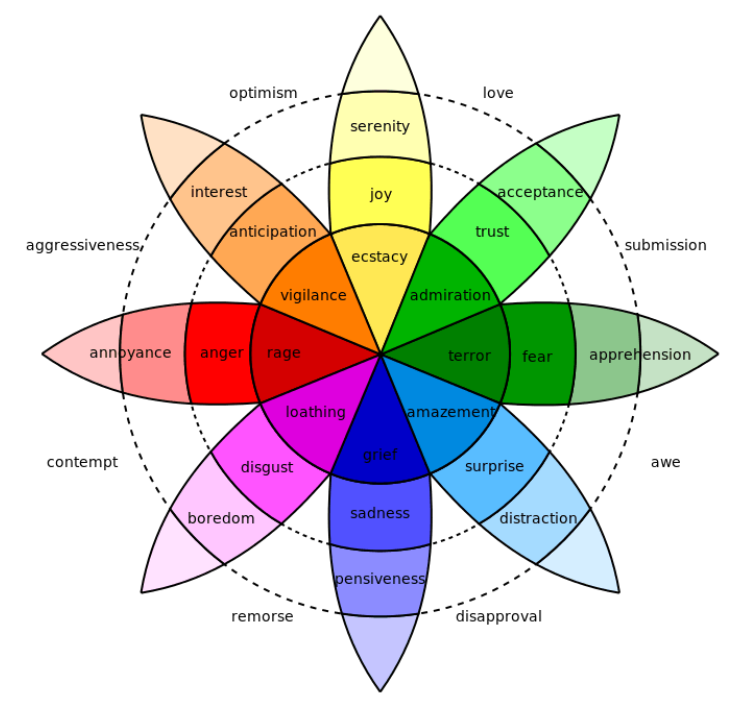
\includegraphics[width=0.5\textwidth]{./img/nlp/emozioni.png}
            \caption{Classificazione delle emozioni}
            \label{fig:emozioni}
      \end{figure}
\end{definizione}
\subsection{Rappresentazione del testo}
Il primo passo consiste nel capire come rappresentare il testo. Questo passaggio
è necessario per passare da una misura qualitativa a una misura quantitativa.

Una prima soluzione è quella di rappresentare il testo tramite un dizionario
di parole. Questo metodo è molto semplice e permette di rappresentare il testo
come un vettore di bit, dove il bit $i$-esimo è a $1$ se la parola $i$-esima
è presente nella frase. Questo metodo però ha dei problemi:
\begin{itemize}
      \item Il vettore che rappresenta la frase è molto grande e sparso.
      \item Perdiamo l'ordinamento delle parole.
\end{itemize}
Un ulteriore metodo è rappresentato dalla \textbf{BagOfWord}, la quale consiste
nel rappresentare una frase tramite un vettore in uno spazio. Il problema è che
manca la composizionalità delle parole.

Possiamo usare una rappresentazione deep basata su \textbf{word2vec}. Questa consiste
nello scrivere il termine sulla base dei termini che lo precedono e che lo seguono.
Si ha quindi uns strategia simile alla BagOfWord, ma mantenendo la composizionalità.

Word2Vec è un modello che viene usato per creare una rappresentazione vettoriale
delle parole. Questo modello è basato su una rete neurale che prende in input
una parola e cerca di prevedere le parole che la circondano.
\begin{itemize}
      \item \textbf{skip-gram}: parte da una parola del documento e cerca di
            predire l'intorno della parola.

            Per ottenere questo risultato, usiamo un \textbf{one-hot-vector},
            ovvero un bitvector, lungo quanto il il vocabolario, con un bit a $1$
            nella posizione associata alla parola all'interno del vocabolario.

            Successivamente costruiamo una rete neurale (Encoder Decoder) che
            preso in input il bitvector, in output dobbiamo avere un vettore
            lungo tanto quanto il vocabolario con una probabilità associata ad
            ogni parola. La rappresentazione vettoriale coincide con  quello che
            si ha nell'hidden layer, la sua dimensione è decisa in fase di
            costruzione della rete.

            Il documento viene rappresentato dal vettore media dei vettori dei
            termini presenti nel documento.

            A differenza dalle rappresentazioni più vecchie abbiamo un vettore di
            dimensione $n$ selezionato dalla rete. Il problema è che non consideriamo
            il contesto del mondo.

            Esistono metodi più efficaci per rappresentare il testo come
            \textbf{USE} e \textbf{BERT}.
      \item \textbf{CBOW}: cerca di predire la parola sulla base dell'intorno
            delle parole vicine.
\end{itemize}
Questi permettono di avere parole con lo stesso significato o simili vicine nello
spazio vettoriale.

Una volta risolto il problema della rappresentazione si può passare alla fase
di classificazione. Questa può essere fatta in diversi modi:
\begin{itemize}
      \item \textbf{Lexicon-based}: si basa su un dizionario di parole associate
            a delle emozioni. Si contano le parole associate alle emozioni e si
            restituisce l'emozione con il conteggio maggiore. Se le emozioni hanno
            lo stesso numero di parole allora la frase è neutra.
      \item \textbf{Machine Learning}: si basa su un modello di classificazione
            che prende in input il vettore che rappresenta la frase e restituisce
            l'emozione.
\end{itemize}
\begin{nota}
      Nel primo caso risulta importate scegliere bene il lessico, perché le parole
      possono essere positive o negative in base al contesto.
\end{nota}

\section{Semantic Ambiguity}
 (disambiguazione dal punto di vista morfosintattico)
Uno dei tanti problemi che si riscontrano nell'analisi del linguaggio naturale
è l'ambiguità delle parole. Questo è molto importante, in quanto per comprendere
un testo bisogna capire a che cosa ogni token si riferisce.

I problemi che si possono riscontrare nel riconoscimento dei token sono riportati
di seguito:
\begin{enumerate}
      \item Il linguaggio con cui è scritto il testo è \textbf{rumoroso}, ovvero
            sono presenti errori ortografici, ambiguità e polisemia (a una parola
            posso associare più significati).
      \item \textbf{Out of vocabulary} (OOV): quando il modello non ha mai
            incontrato delle parole che gli vengono fornite come input. Ad esempio,
            se in fase di training il modello ha appreso la frase ``The Big Bang
            Theory'', mentre in fase di test gli viene fornita la frase ``TBBT'',
            il modello non riconoscerà la parola.
      \item \textbf{Out of Knowledge base}: quando il modello non ha una
            rappresentazione dell'entità nella base di conoscenza. Ad esempio,
            il nome di un nuovo prodotto.
\end{enumerate}
\subsection{Name entity recognition}
\begin{definizione}[\textbf{Named Entity Recognition}]
      La \textbf{Named Entity Recognition} (NER) è una tecnica che permette di
      identificare le entità all'interno di un testo e classificarle in categorie
      predefinite.
\end{definizione}
\begin{definizione}[\textbf{Surface Form}]
      La \textbf{Surface Form} è la rappresentazione di un'entità indipendente
      dalla semantica nella frase.
\end{definizione}
Per svolgere questo task si utilizzano dei modelli neurali i quali escono dalla
classica idea di machine learning, in quanto l'output non è più un singolo valore
ma una sequenza di valori. Questo problema viene risolto con i modelli \textbf{sequence
      prediction}.

Nel nostro caso si ha una sequenza di osservazioni e si impara per prevedere la
sequenza ottimale di etichette che devono essere associate alle osservazioni.
In questo modo si considera nella predizione il contesto delle osservazioni
facenti parte della sequenza, quindi non si effettua il training sulle singole parole.
\subsubsection{Conditional Random Fields}
Il modello che viene utilizzato per risolvere il problema di NER è il \textbf{Conditional
      Random Fields} (CRF). Questo modello è un modello grafico probabilistico che
massimizza la probabilità condizionata delle etichette della sequenza di input.

Questo modello può essere come un grafo dove si hanno dei nodi che rappresentano
le osservazioni e degli archi che rappresentano le dipendenze tra le etichette.

Le parole sono connesse solamente alle etichette, mentre è presente una relazione
temporale tra le etichette. Questo modello è un modello di Markov del primo ordine,
in quanto si considera solamente la parola precedente.

Vediamo ora un esempio di struttura di un CRF:
\begin{figure}[!ht]
      \centering
      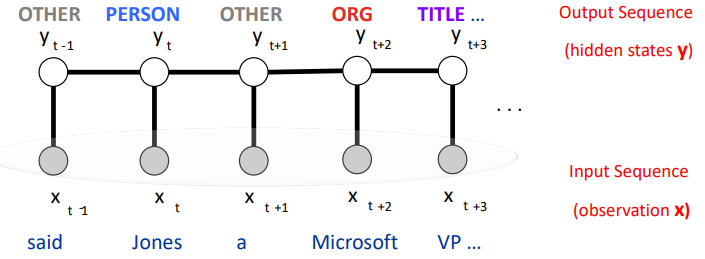
\includegraphics[width=0.5\textwidth]{./img/nlp/crf.png}
      \caption{Struttura di un CRF}
      \label{fig:crf}
\end{figure}

In fase di training si impara $P(y|x)$, dove $y$ è il vettore delle etichette
mentre $x$ è il vettore delle parole.
\begin{equation}
      P(y|x) = \frac{1}{Z_x} \prod_t \phi(y_t,y_{t-1},x ,t)
\end{equation}
dove $\frac{1}{Z_x}$ rappresenta una costante di normalizzazione, mentre la
funzione $\phi(y_t,y_{t-1},x ,t)$ può essere scritta come:
\begin{equation}
      \phi(y_t,y_{t-1},x ,t) = \exp (\sum_k\lambda_k f_k(y_t,y_{t-1},x,t))
\end{equation}
dove $f_k(y_t,y_{t-1},x,t)$ sono delle \textbf{feature function}, ovvero delle
funzioni predeterminate che valutano diverse proprietà in base all'osservazione e
all'etichetta precedente al tempo $t$.È impor tante che queste funzioni abbiano
almeno due stati di uscita, possiamo considerare le feature function come degli
\textbf{if}.

Le feature function possono essere di due tipologie:
\begin{itemize}
      \item \textbf{State} $f_i(y_t, x) \in \mathbb{R}$: valutano lo stato in
            cui ci si trova in quel tempo. Nello specifico valutano la relazione
            che c'è tra la parola $x_t$ e la sua etichetta $y_t$.
      \item \textbf{Transition} $g_i(y_t, y_{t - 1}, x) \in \mathbb{R}$: modellano
            la dinamica dell'etichettatura. Misurano la relazione tra l'etichetta
            della parola al tempo $t$ e l'etichetta della parola al tempo $t - 1$.
            Le definisco a runtime perché si applicano alle etichette.
\end{itemize}

Quanto ottenuto è un modello log-lineare, quindi, possiamo riscrivere il calcolo
della probabilità condizionata come:
\begin{equation}
      P(y|x) = \frac{\exp \sum_{t = 1}^T\left( \sum_i \lambda_i f_i(y_t,x) +
      \sum_j \mu_j g_j(y_t,y_{t-1},x) \right)}{Z_x}
\end{equation}
Dato che le funzioni sono note, dobbiamo imparare i parametri $\lambda_i, \mu_j$,
per fare questo, si massimizza la \textbf{log-likelihood} del modello rispetto
alle osservazioni, ovvero:
\begin{equation}
      L_{\lambda,\mu} = \sum_{t} \log P(y_t|x_t, \lambda, \mu) = \sum_k \left[
            (\lambda, \mu) \cdot F(y_k, x_k) - \log Z_{\lambda, \mu}(x_k) \right]
\end{equation}
L'inferenza consiste nel determinare la migliore sequenza di etichette data una
sequenza di osservazioni.

Il processo di inferenza avviene tramite l'algoritmo di \textbf{Viterbi}, il quale
trova la sequenza di etichette che massimizza la probabilità condizionata. Si ha
una struttura simile a una rete neurale, dove ogni layer è composto da tanti nodi
quante le etichette possibili. La rete e fully connected e ogni arco ha un peso
associato, determinato dalla feature function.

La valutazione del modello si effettua in due metodologie:
\begin{itemize}
      \item \textbf{Exact Match}: considero corretta la predizione se tutta l'entità
            viene riconosciuta correttamente. Utile se devo fare sentiment analysis.
      \item \textbf{Partial Match}: considero corretta la predizione se l'entità
            viene riconosciuta parzialmente. Utile se devo fare retrival del db.
\end{itemize}
\subsection{Named Entity Linking}
Una volta riconosciuta l'entità spesso si effettua \textbf{named-entity linking},
ovvero partendo dalla surface form si cerca di associare l'entità ad una risorsa
presente nella base di conoscenza.

Questo task viene svolto nel seguente modo:
\begin{enumerate}
      \item Si cerca nella base di conoscenza il token usando la sua surface form.
      \item Si prendono i primi $k$ risultati e si calcola la similarità tra
            la surface form e il risultato. Questo può essere fatto tramite
            diverse metriche e considerando diversi attributi.
      \item Si restituisce l'entità con la similarità maggiore.
\end{enumerate}

Un esempio di pipeline per il name entity linking è riportato di seguito:
\begin{figure}[!ht]
      \centering
      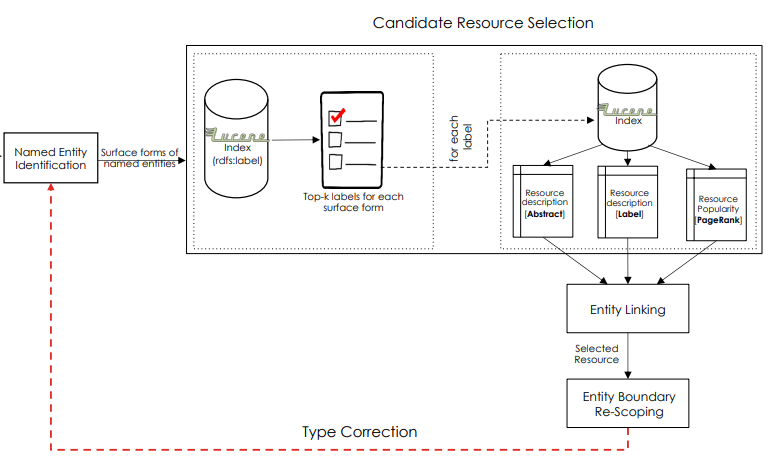
\includegraphics[width=0.5\textwidth]{./img/nlp/nel.png}
      \caption{Pipeline per il Named Entity Linking}
      \label{fig:nel}
\end{figure}
\subsection{Word sense disambiguation}
Si cerca di comprendere il significato della parola che è accettato comunemente.
Questo ci permette di disambiguare il significato della parola dal punto di
vista del senso. Dobbiamo però considerare che il significato della parola può
dipendere da quello che la circonda.

Gli approcci che possono essere utilizzati per risolvere questo problema sono:
\begin{itemize}
      \item \textbf{Knowledge-based Disambiguation}: sono sistemi basati su basi
            di conoscenza, come dizionari e tesauri.
      \item \textbf{Supervised Disambiguation}: sono sistemi che richiedono dati
            etichettati per funzionare.
      \item \textbf{Unsupervised Disambiguation}: sono sistemi che non richiedono
            dati etichettati per funzionare.
\end{itemize}
\subsubsection{Knowledge-based Disambiguation}
Nei metodi basati su basi di conoscenza, la disambiguazione della parola si
effettua tramite un dizionario machine readable e dati raw. Non servono quindi
dei dati etichettati e si lavora su parole appartenenti alle open class.

Nei dizionari si possono trovare molte informazioni utili per la disambiguazione,
possiamo trovare i sinonimi, le definizioni, le relazioni tra le parole, etc.

Un primo algoritmo è \textbf{Lesk algorithm}, definisce il senso delle parole
nel contesto confrontando le definizioni si sovrapposizioni. Il funzionamento di
questo algoritmo è il seguente:
\begin{itemize}
      \item Prende dai machine readable dictionary le definizioni di tutte le
            parole che si vogliono disambiguare.
      \item Determina gli overlap tra tutte le coppie di parole da disambiguare.
      \item Seleziona il significato in base al massimo numero di overlap.
\end{itemize}
Questo algoritmo è molto pesante dal punto di vista computazionale in quanto
si devono calcolare tutte le combinazioni di parole.

Per questo motivo, è stata introdotta una variante detta \textbf{Simplified Lesk}
il quale funziona nel seguente modo:
\begin{itemize}
      \item Prende dai machine readable dictionary le definizioni della parola
            che si vuole disambiguare.
      \item Calcola l'overlap tra la parola da disambiguare e tutte le altre
            della frase.
      \item Seleziona il significato con il massimo overlap.
\end{itemize}